\documentclass[aspectratio=169]{beamer}
\usepackage{minted}
\usepackage{listings}
\usetheme{veit}
\title{SCHEME: An Interpreter for Extended Lambda Calculus}
\subtitle{Gerald J. Sussman and Guy L. Steele Jr.}
\date{\today}
\author{Veit Heller}
\institute{Papers We Love Berlin}
\begin{document}
  \maketitle
  \begin{frame}{Agenda}
    \begin{itemize}
      \item Introduction and historical context
      \item Scheme primer
      \item A “hairy control structure”
      \item Let’s see some code!
      \item Implementation notes
    \end{itemize}
  \end{frame}
  \begin{frame}{The Paper}
    In 1975, a 21-year-old grad student named Guy Steele and his thesis
    advisor Gerald Sussman had something to show to the world: a little
    programming language called Scheme.

  \end{frame}
  \begin{frame}{The Paper}
    \begin{figure}
      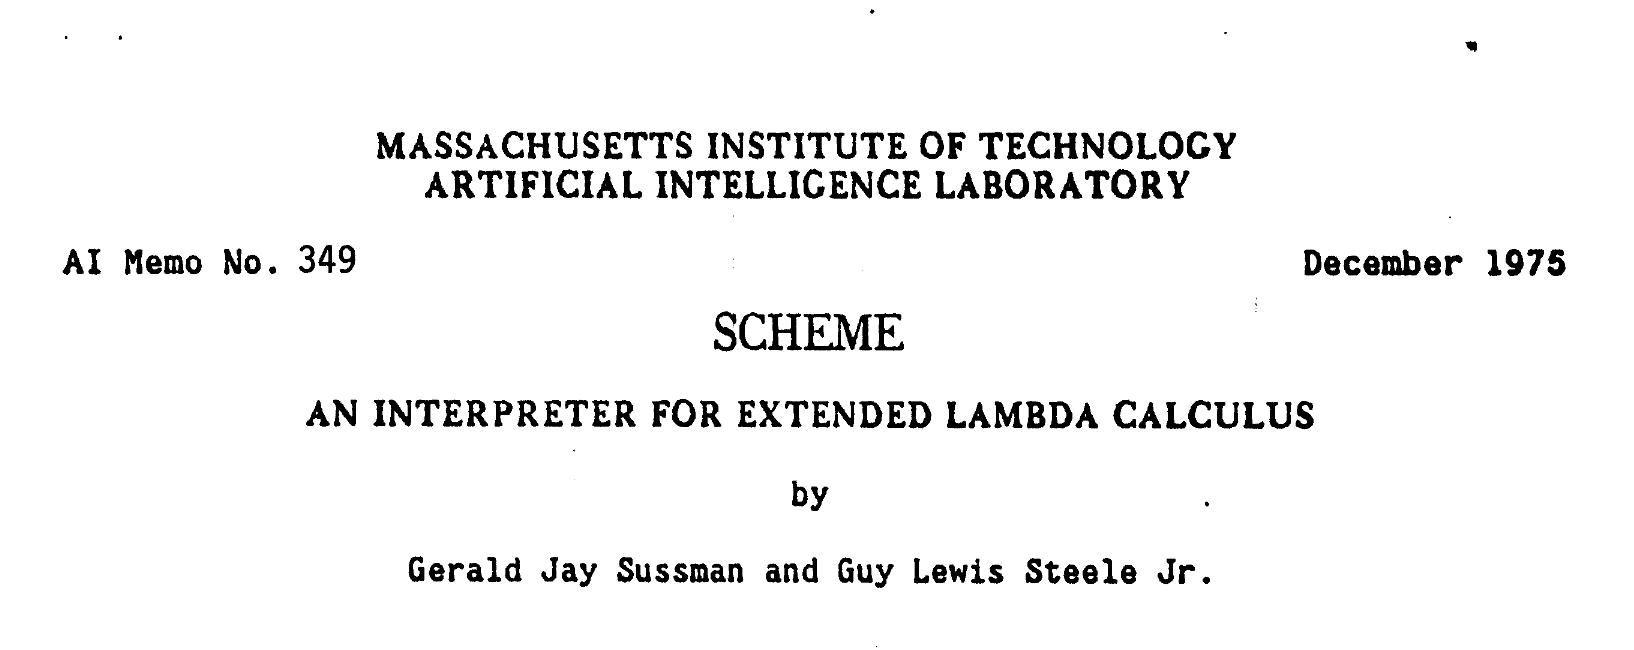
\includegraphics[width=\linewidth]{header.png}
      \caption{A wild paper appears.}
    \end{figure}
  \end{frame}
  \begin{frame}{The Paper}
    The paper has all the goods a hacker could wish for: a reference, cool code
    examples, and an implementation of Lisp in Lisp.
  \end{frame}
  \begin{frame}{The Name}
    The language was originally intended to be called SCHEMER, in reference
    to its ancestors PLANNER and CONNIVER.
  \end{frame}
  \begin{frame}[fragile]
    \frametitle{Scheme: A primer}
    In Scheme, we define functions using \textit{define}—you might know it as
    \textit{defn} or \textit{defun} in other Lisps:

    \begin{listing}[H]
      \caption{Defining addition}
      \begin{minted}{scheme}
(define add
  (lambda (x y)
    (+ x y)))
      \end{minted}
    \end{listing}

    NB: I eschewed the all-caps notation, and I hope your eyes will thank me
    for it.
  \end{frame}
  \begin{frame}[fragile]
    \frametitle{Scheme: A primer}
    We can \textit{quote} things using either the function or the abbreviation
    \textit{'}.

    \begin{listing}[H]
      \caption{Using symbols as values}
      \begin{minted}{scheme}
; this will always return the symbol x
(define gimme-x (lambda () 'x))
      \end{minted}
    \end{listing}
  \end{frame}
  \begin{frame}[fragile]
    \frametitle{Scheme: A primer}
    There is also the somewhat idiosyncratic \textit{labels}, which allows you
    to define local functions that can be called inside a context, and can call
    themselves and other local functions in that context. You might know it as
    \textit{letrec*} from later Schemes, and as simply \textit{let} in Common
    Lisp.
  \end{frame}
  \begin{frame}[fragile]
    \frametitle{Putting it all together}
    \begin{listing}[H]
      \caption{Let’s define something!}
      \begin{minted}{scheme}
; lets define cells!
(define cons-cell (lambda (contents)
    (labels ((the-cell
                (lambda (msg)
                  (if (eq msg 'contents) contents
                    (if (eq msg 'cell?) 'yes
                      (if (eq (car msg) '<-)
                        (block (aset 'contents (cadr msg))
                               the-cell)
                        (error '|Unrecognized Message - Cell|
                               msg
                               'wrng-type-arg)))))))
      the-cell)))
      \end{minted}
    \end{listing}
  \end{frame}
  \begin{frame}{And now?}
    There is more, though!

    Let’s get to the good stuff.
  \end{frame}
  \begin{frame}
    TODO: Talk about new control structures.
  \end{frame}
  \begin{frame}
    TODO: Talk about code examples: samefringe, pattern matching, multiprocessing.
  \end{frame}
  \begin{frame}
    TODO: Talk about the implementation.
  \end{frame}
\end{document}
